\usepackage{graphicx}
\newpage
\thispagestyle{fancy}
\vspace{\fill}

\subsection{Visão geral dos comandos nas impressoras}
\begin{figure}
    \centering
    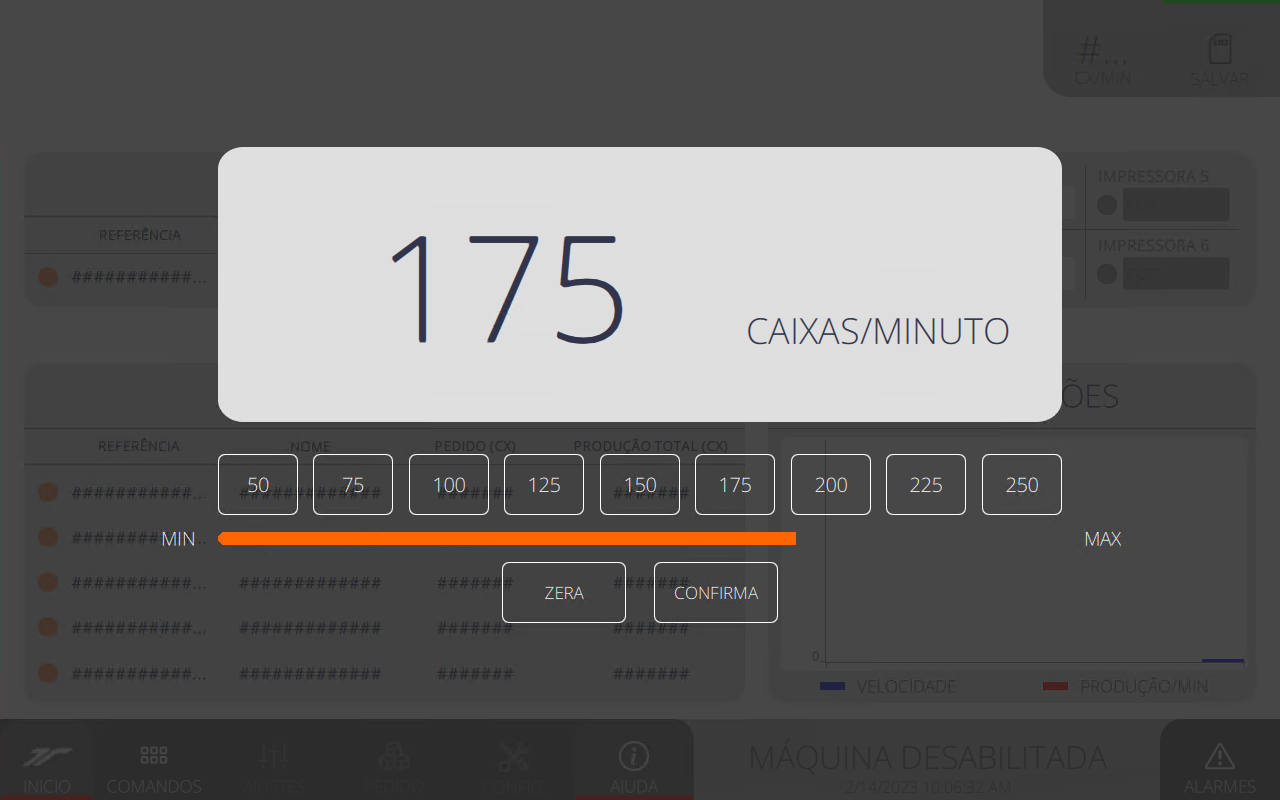
\includegraphics[width=480,height=300]{imagesICV/04-printters/01-printters/commands/1}
    \caption{Visão geral dos comandos nas impressoras}
\end{figure}
\newpage
\thispagestyle{fancy}
\vspace{\fill}

\subsection{Aproximação do anilox bloqueada}
\begin{figure}
    \centering
    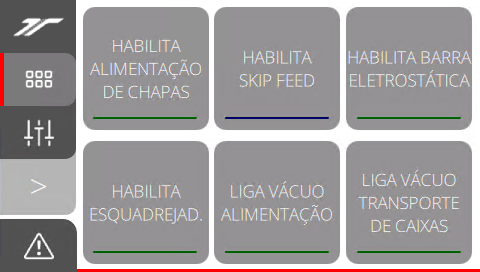
\includegraphics[width=576,height=360]{imagesICV/04-printters/01-printters/commands/2}
    \caption{Aproximação do anilox bloqueada}
\end{figure}
\newpage
\thispagestyle{fancy}
\vspace{\fill}

\subsection{Ventilador de vácuo habilitado}
\begin{figure}
    \centering
    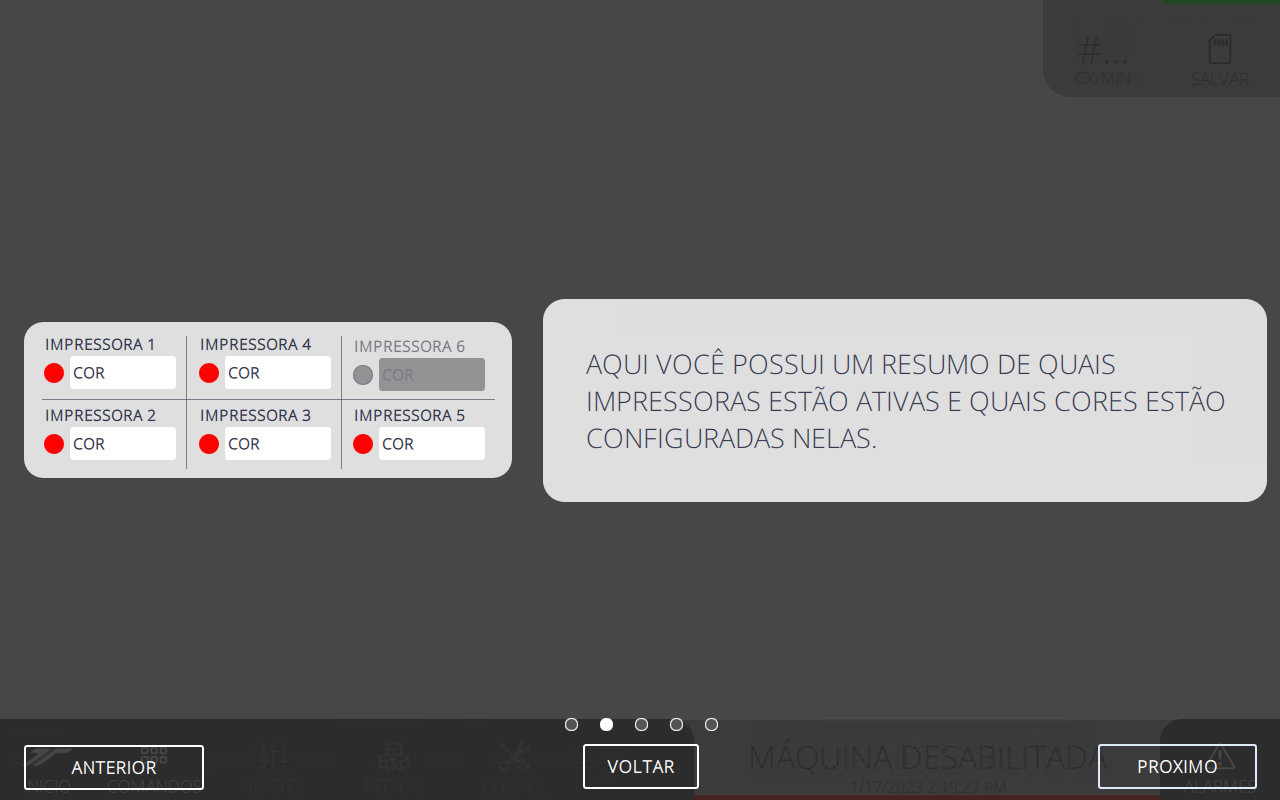
\includegraphics[width=576,height=360]{imagesICV/04-printters/01-printters/commands/3}
    \caption{Ventilador de vácuo habilitado}
\end{figure}
\newpage
\thispagestyle{fancy}
\vspace{\fill}

\subsection{Rolo anilox habilitado}
\begin{figure}
    \centering
    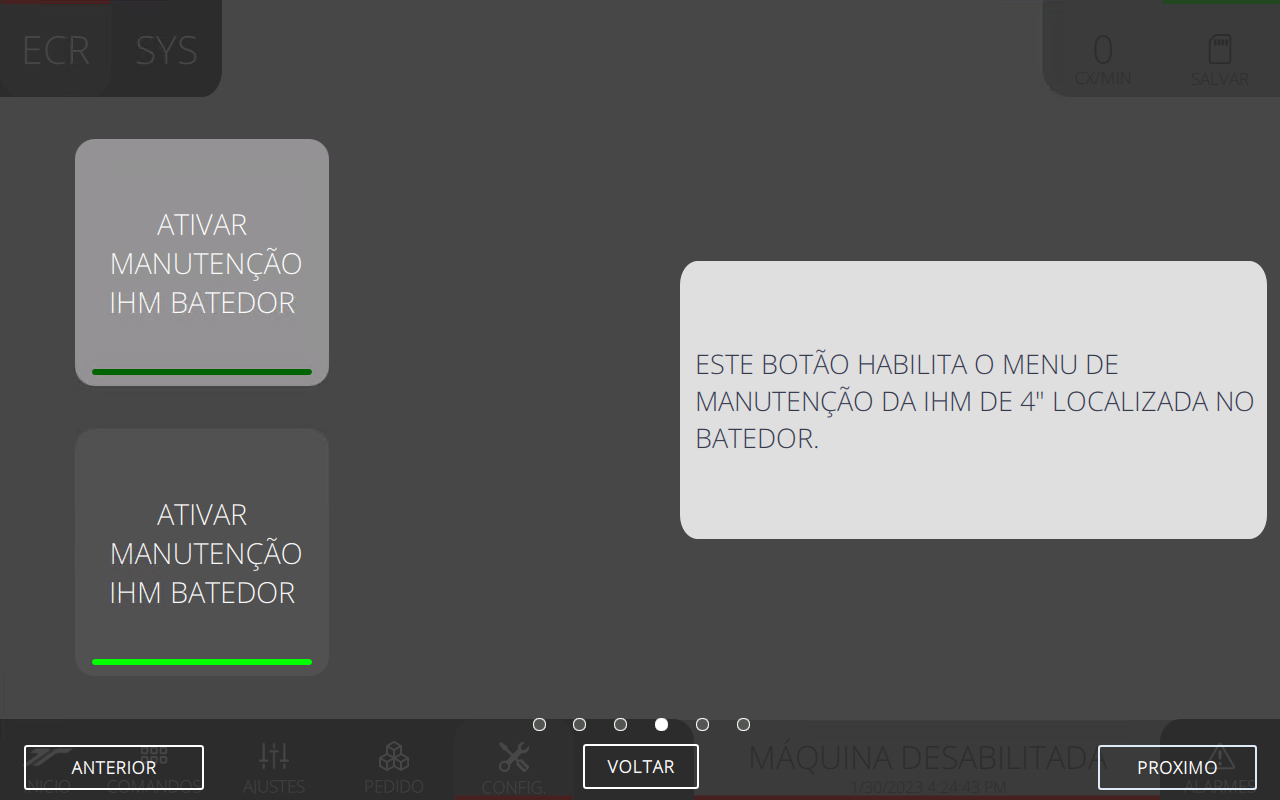
\includegraphics[width=576,height=360]{imagesICV/04-printters/01-printters/commands/4}
    \caption{Rolo anilox habilitado}
\end{figure}
\newpage
\thispagestyle{fancy}
\vspace{\fill}

\subsection{Lavagem de tinta habilitada}
\begin{figure}
    \centering
    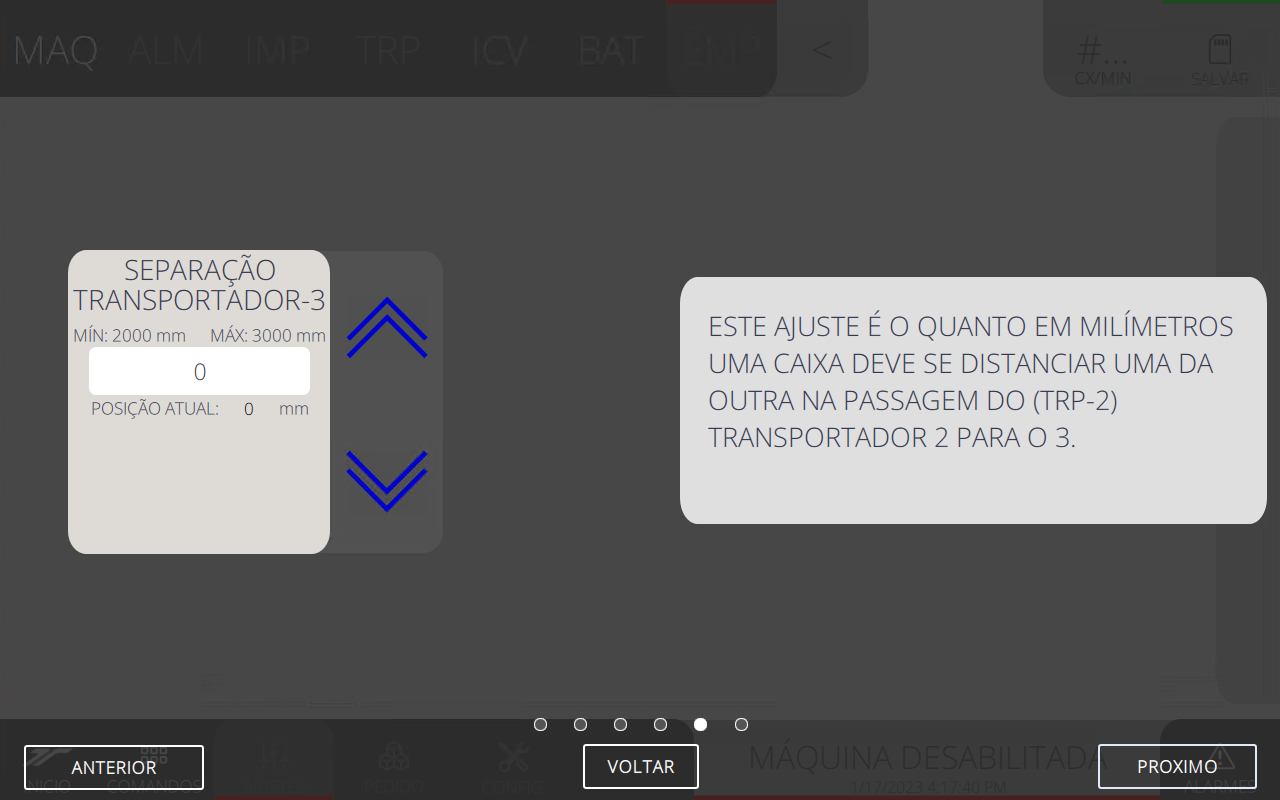
\includegraphics[width=576,height=360]{imagesICV/04-printters/01-printters/commands/5}
    \caption{Lavagem de tinta habilitada}
\end{figure}
\newpage
\thispagestyle{fancy}
\vspace{\fill}

\subsection{Unidade travada}
\begin{figure}
    \centering
    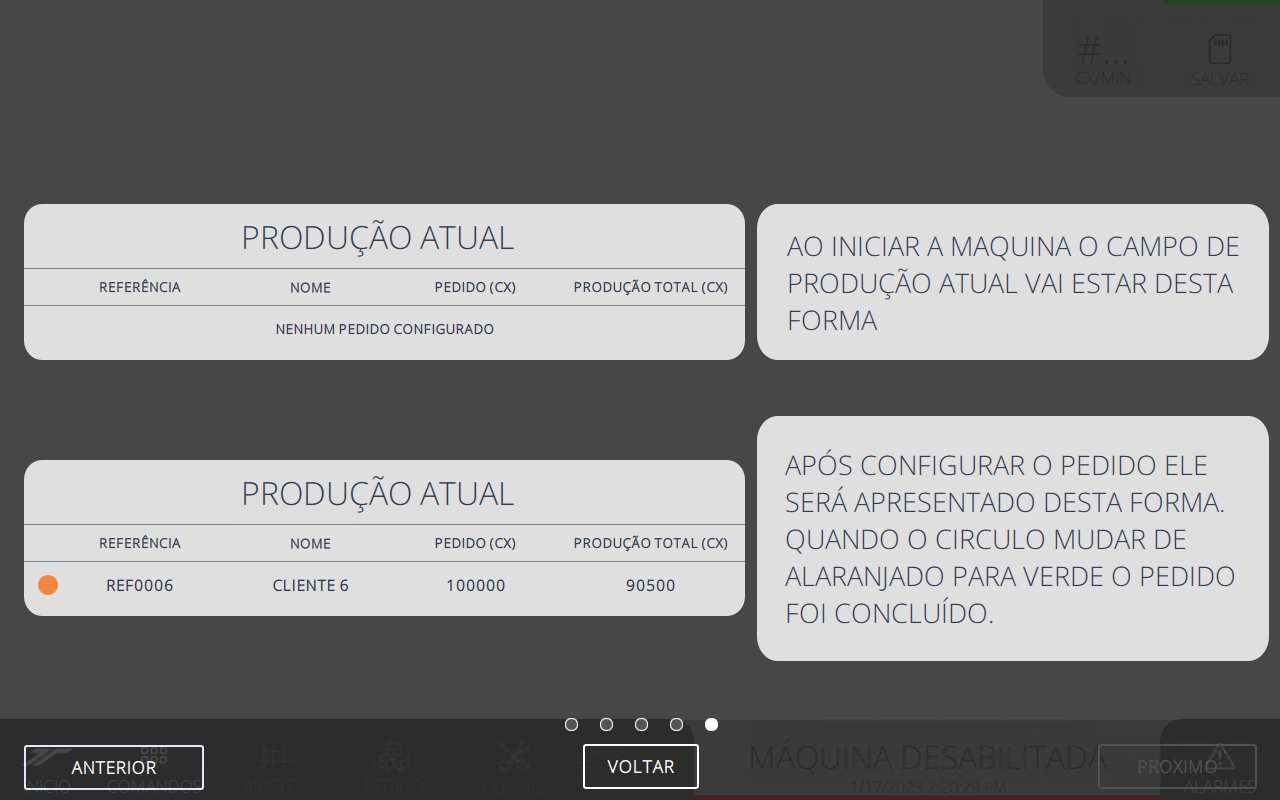
\includegraphics[width=576,height=360]{imagesICV/04-printters/01-printters/commands/6}
    \caption{Unidade travada}
\end{figure}
\newpage
\thispagestyle{fancy}
\vspace{\fill}

\subsection{Acesso à tela de comamndo da unidade}
\begin{figure}
    \centering
    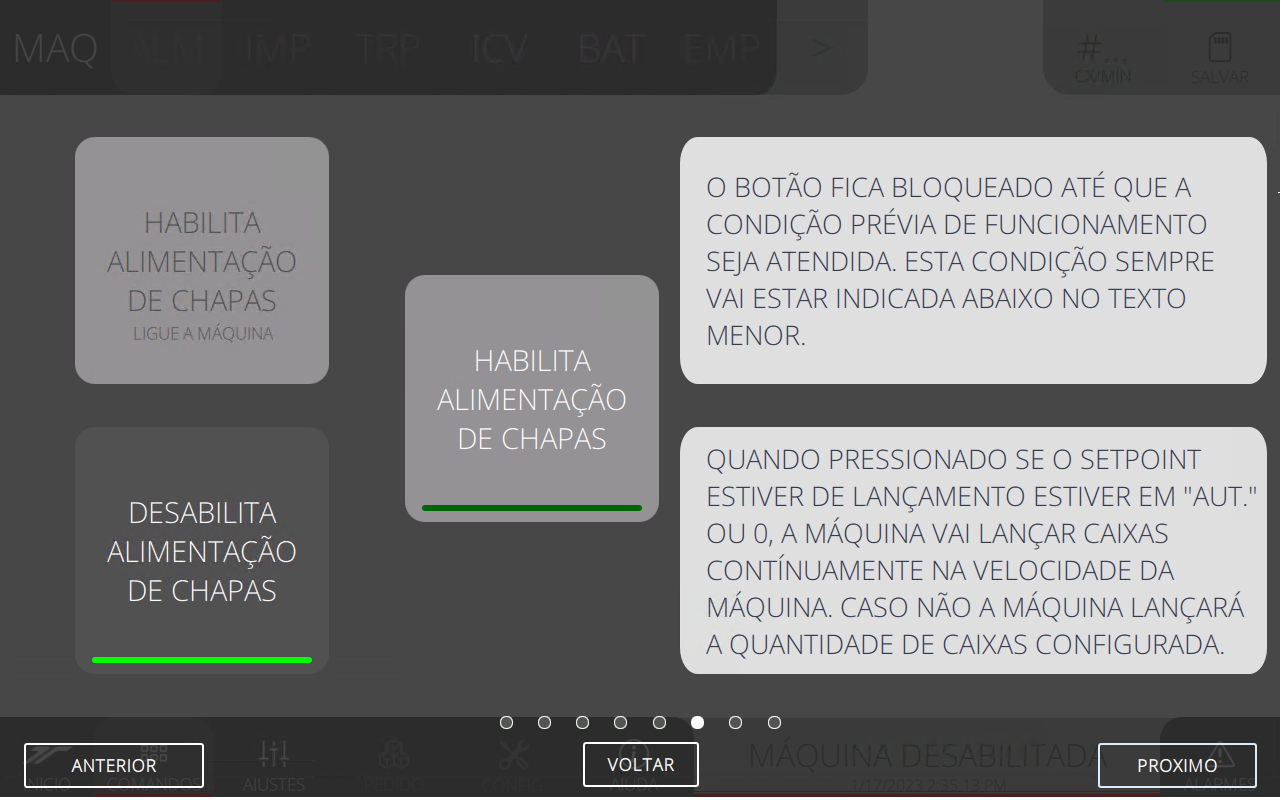
\includegraphics[width=576,height=360]{imagesICV/04-printters/01-printters/commands/7}
    \caption{Acesso à tela de comando da unidade}
\end{figure}


